For \dword{ce} development, testing prototypes at room temperature is the first step, as many problems can be identified quickly and without the expense of cryogens.  A quick access test stand with the \dword{femb} connected to an \dword{apa} inside a shielded environment that is in the same location as the \dword{femb} and \dword{asic} development is invaluable for rapid progress.  Two such facilities are available to DUNE: the shielded room at \fnal and the \num{40}\,\% \dword{apa} test stand at BNL.  In addition, a test dewar design developed by Michigan State University, referred to as the Cryogenic Test System (CTS), allows for additional testing of the \dwords{femb} and \dwords{asic} in LN$_2$.

The shielded room at \fnal (see Figure~\ref{fig:shieldedroom}) is \SI{2.5}{m} tall, and \SI{2}{m} on each side, with 
a double layer of copper mesh in the walls, floor and ceiling, plus a solid metal plate in the floor all electrically connected to create a Faraday cage.  A flexible AC distribution and isolated grounding configuration offers the ability to easily ground the shielded room and refer the associated electronics to either a building ground or a detector ground.  In addition
to evaluating different grounding schemes for the \dwords{apa}, capacitive coupling issues can be studied by varying the
distance between the floor and a copper plate positioned underneath.   
This room has uniquely easy access to the setup through a shielded door,
and a person can remain inside safely with the door closed and probe the electronics directly while operating
in a shielded environment.  Currently mounted inside are two \dwords{apa} from the \SI{35}{t} 
with adapter boards to connect \dword{pdsp} electronics.  This installation satisfies the \dword{pdsp} grounding and shielding guidelines.  A rough demonstration of the shielding adequacy for our purposes  is the measured noise level of 800~\dword{enc} for \dword{pdsp} prototype \dwords{femb}.  The same noise level was measured at room temperature in the \num{40}\,\% \dword{apa} at BNL for the same \dwords{femb}.

\begin{dunefigure}
[Picture of the shielded room at \fnal.]
{fig:shieldedroom}
{Picture of the shielded room at \fnal.}
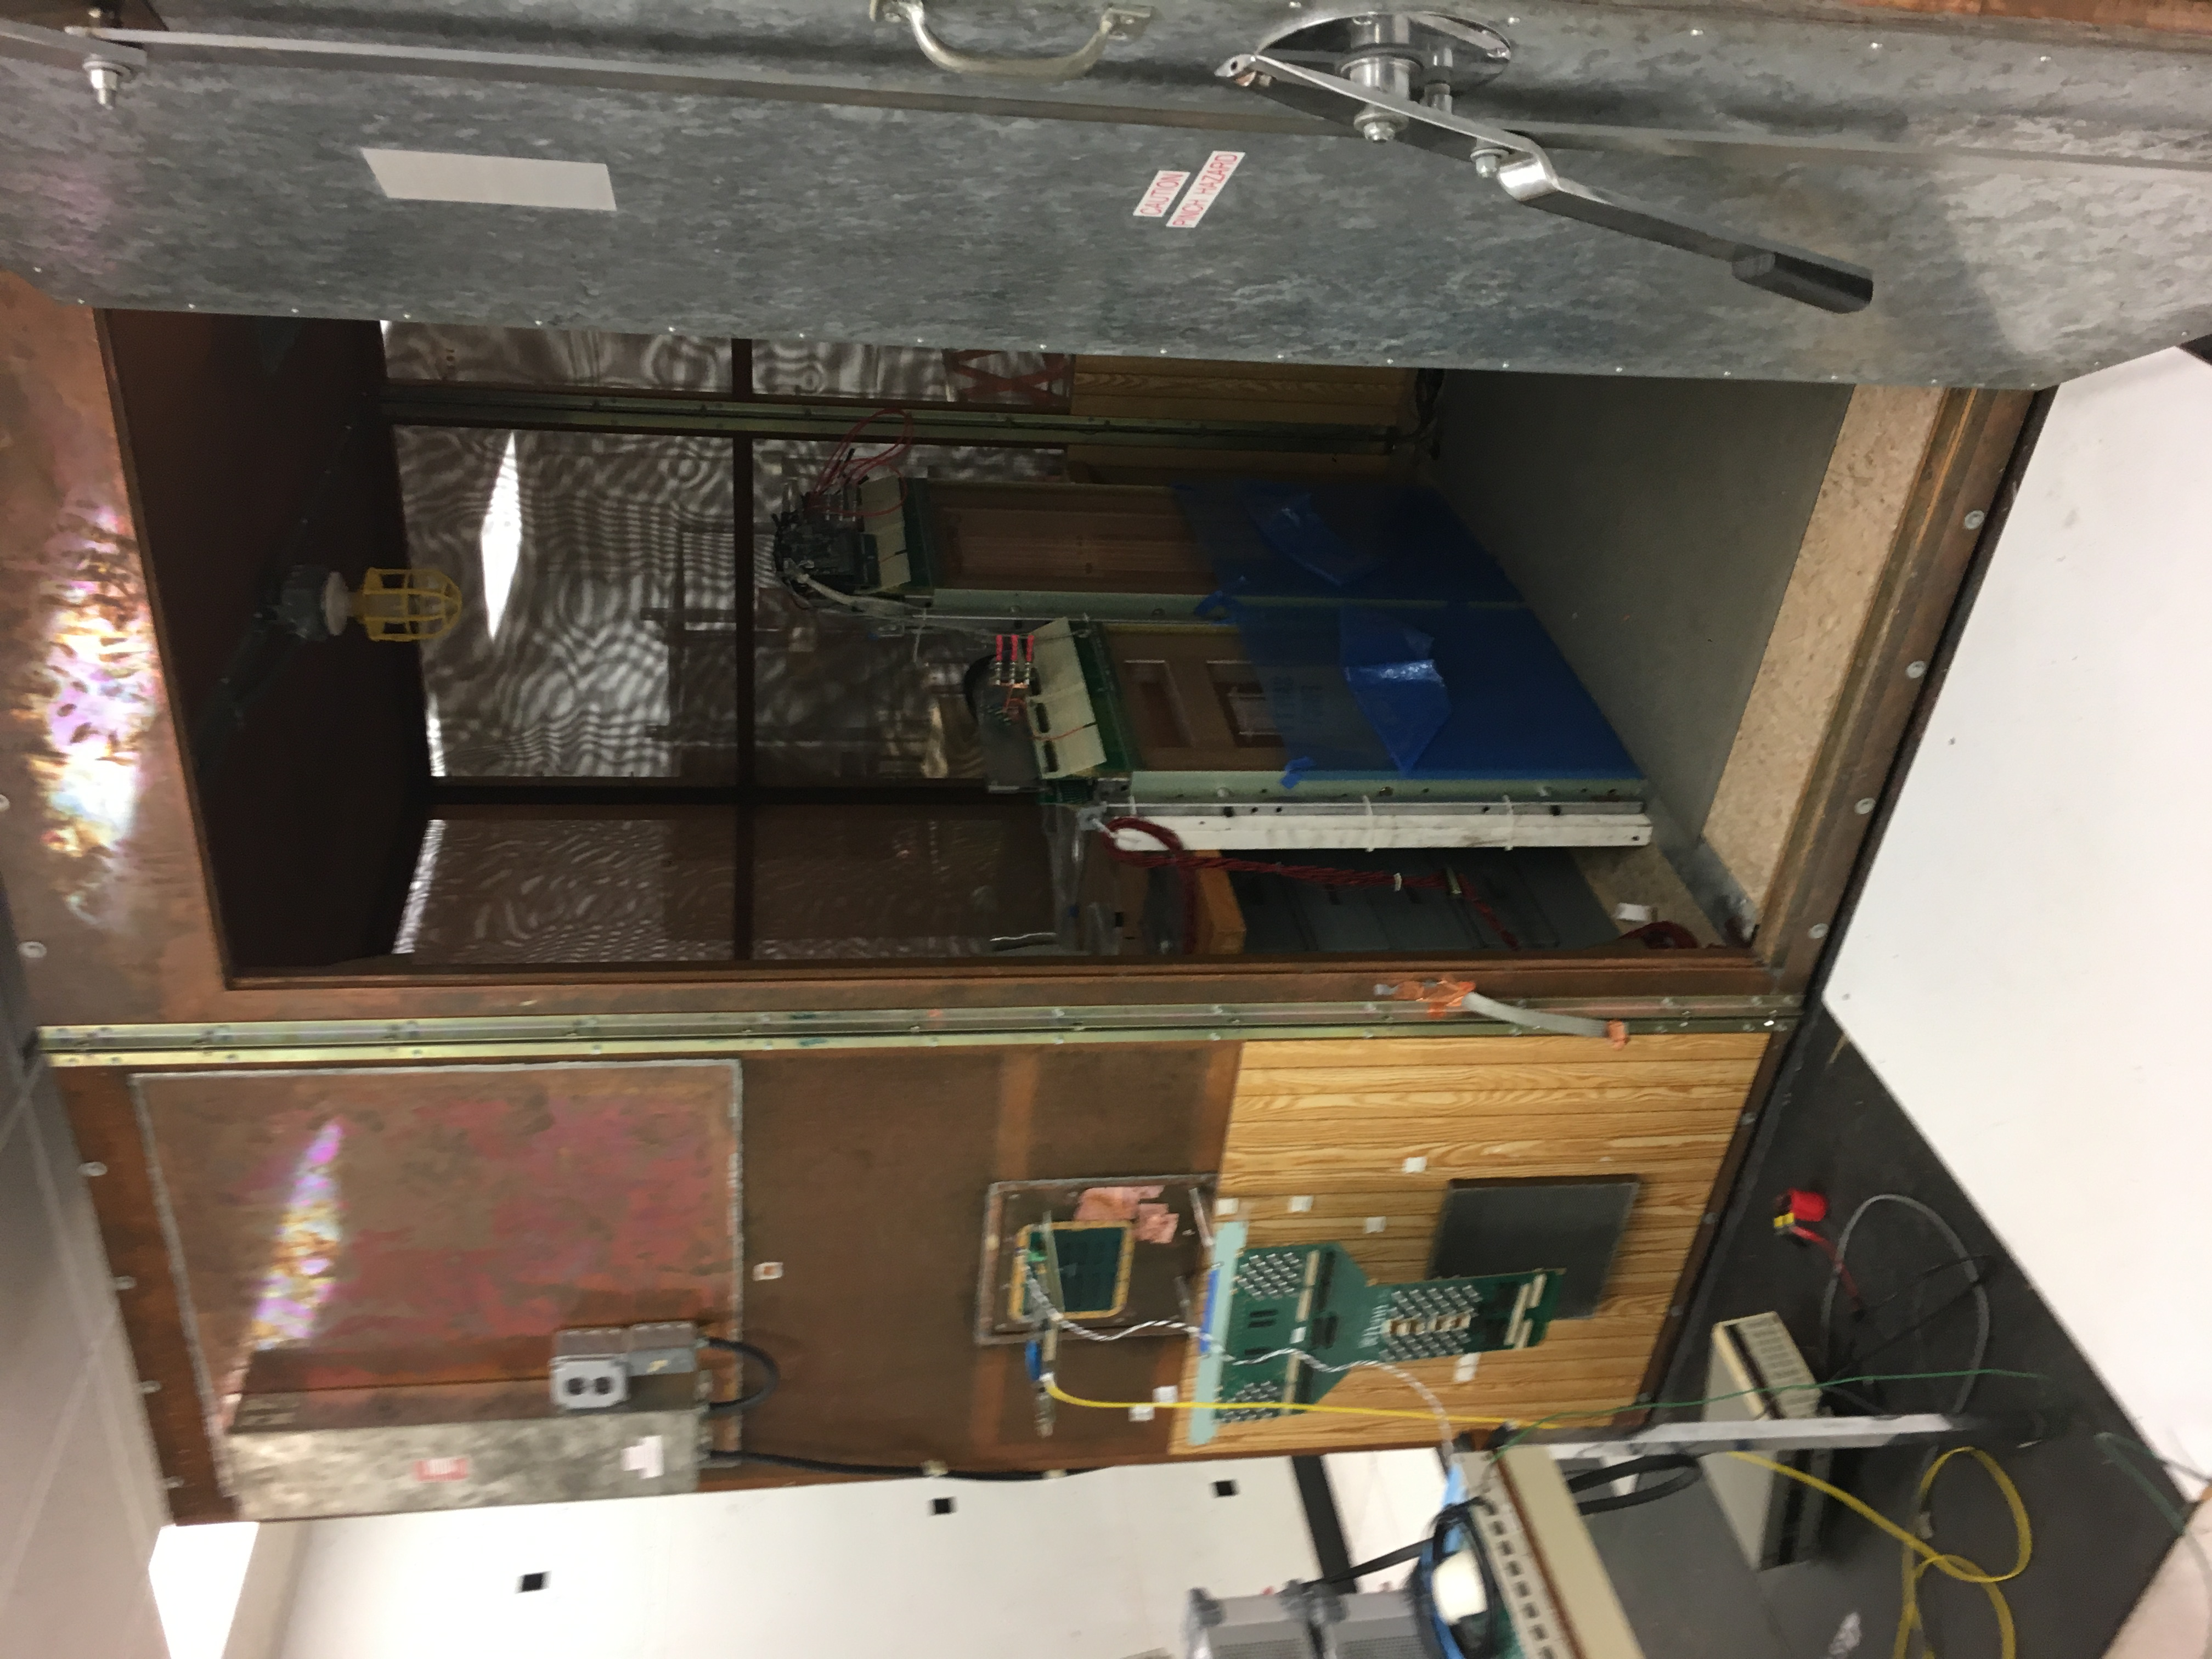
\includegraphics[angle=270,width=0.4\linewidth]{tpcelec-shielded_room.jpg}
\end{dunefigure}

The \num{40}\,\% \dword{apa} at BNL is a \SI{2.8}{m}~$\times$~\SI{1.0}{m} three-plane \dword{apa} with two layers of \num{576} wrapped ($U$ and $V$) wires and one layer of \num{448} straight ($X$) wires. It is read out by eight \dword{pdsp} \dwords{femb} with the full \SI{7}{m} \dword{pdsp} length data and \dword{lv} power cables, four on the top and four on the bottom. The readout uses the full \dword{ce} system for \dword{pdsp}, with a prototype \dword{ce} flange and \dword{wiec}, two \dwords{wib} and one \dword{ptc}, as shown in Figure~\ref{fig:tpcelec_40apa}. Detailed integration tests of the \dword{ce} readout performance while following the DUNE grounding and shielding guidelines have been done at the \num{40}\,\% \dword{apa}. Additional input capacitance (equivalent to longer wire length) have been added to a subset of channels to project the \dword{enc} performance from the 40\% \dword{apa} teststand to the \dword{pdsp} and SBND detectors. The results from the \num{40}\,\% \dword{apa} indicate that, if the new \dword{adc} performs as expected, the full \dword{ce} system as installed on the test  stand at BNL will have a noise level in \lar around \num{500}\,e$^-$ and \num{600}\,e$^-$ for the collection and induction plane channels, respectively, in line with the CERN cold box tests described in Section~\ref{sec:fdsp-tpc-elec-qa-facilities-coldbox}.

\begin{dunefigure}
[One side of the \num{40}\,\% \dword{apa} with four \dwords{femb} and the full \dword{ce} \fdth and flange.]
{fig:tpcelec_40apa}
{Left: one side of the \num{40}\,\% \dword{apa} with four \dwords{femb}.  Right: the full \dword{ce} \fdth and flange.}
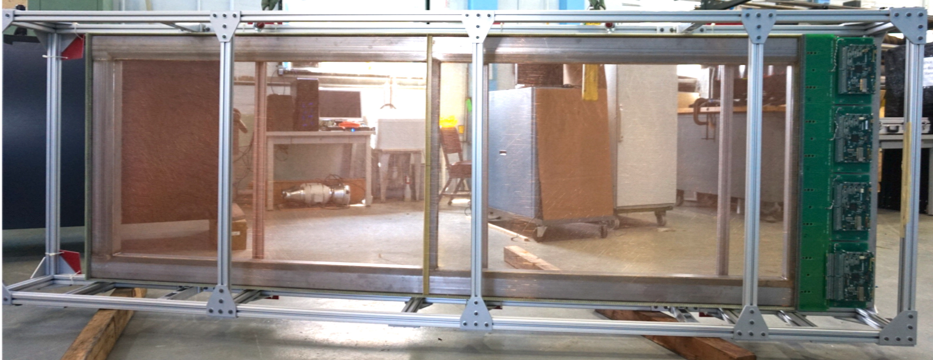
\includegraphics[width=0.72\linewidth]{tpcelec-40-apa.png}
\hspace{3mm}
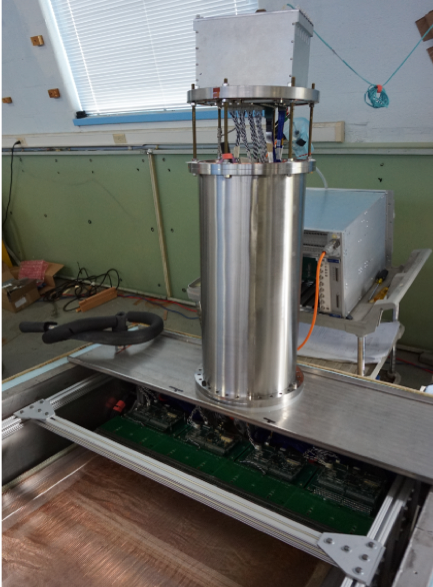
\includegraphics[width=0.2\linewidth]{tpcelec-40-apa-ft.png}
\end{dunefigure}

%\begin{figure}
%    \centering
%    \includegraphics[width=0.9\linewidth]{tpcelec-40-apa-result.png}
%    \caption{\dword{enc} (in electrons) as a function of input capacitance (equivalent to input wire length) measured on the 40\% \dword{apa}. The \dword{enc} projections are based on the input wire length of the SBND and \dword{pdsp} detectors.}
%    \label{fig:tpcelec_40\dword{apa}_results}
%\end{figure}

To facilitate testing of individual components and printed circuit boards, members of the Michigan State group have developed the CTS (see Figure~\ref{fig:CTS}).  This system allows a device under test to be cooled down in nitrogen gas, immersed in LN$_2$ for testing, and then warmed back to room temperature in a nitrogen gas.  This process avoids the condensation of water from air that can otherwise interfere with the tests or damage the test equipment.  A total of nine CTSs will be built and used at consortium member institutions.

\begin{dunefigure}
[The Cryogenic Test System (CTS)]
{fig:CTS}
{Cryogenic Test System: an insulated box is mounted on top of a commercial LN$_2$ dewar.  Simple controls allow the box to be purged with nitrogen gas and LN$_2$ to be moved from the dewar to the box and back to the dewar.}
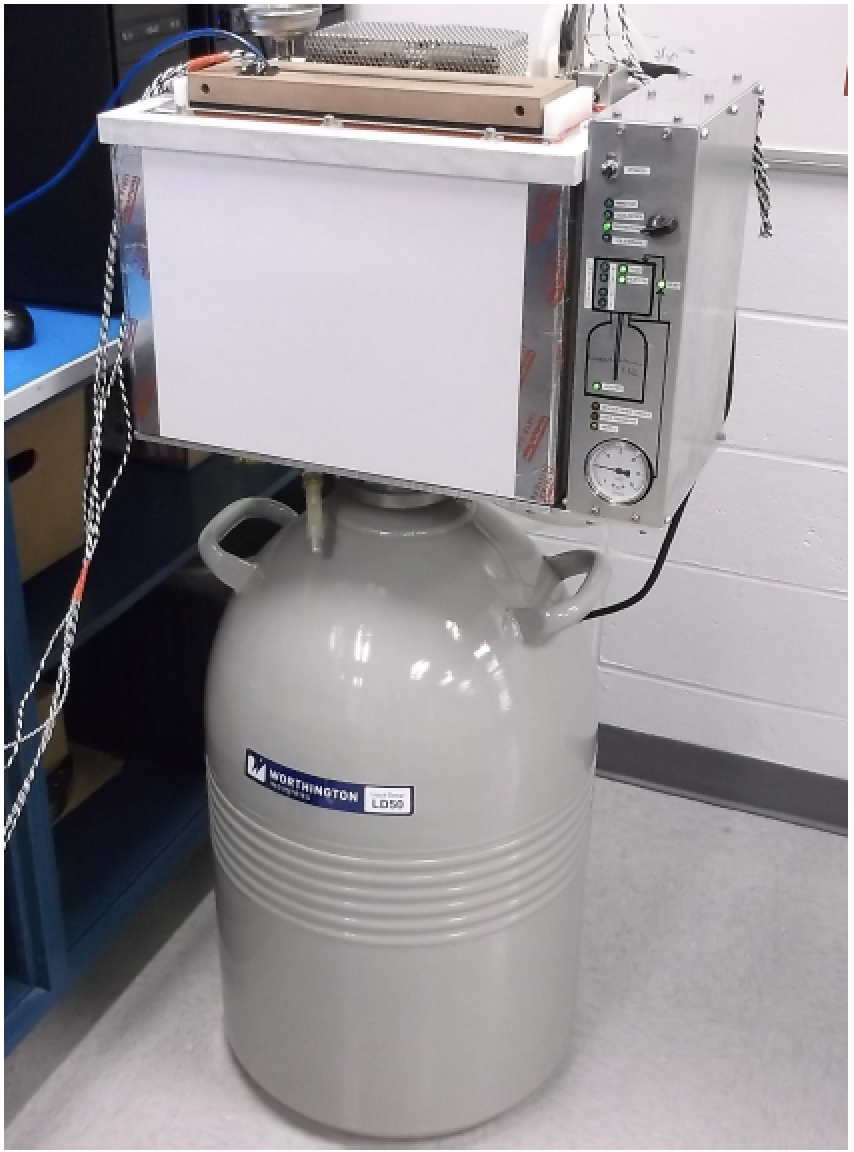
\includegraphics[width=0.4\linewidth]{tpcelec-CTS.png}
\end{dunefigure}
